%%%%%%%%%%%%%%%%%%%%%%%%%%%%%%%%%%%%%%%%%
% Structured General Purpose Assignment
% LaTeX Template
%
% Original author:
% Ted Pavlic (http://www.tedpavlic.com)
%
% modified by Xian Kevin Shi
% University of California, Berkeley
% 2014 Fall
%%%%%%%%%%%%%%%%%%%%%%%%%%%%%%%%%%%%%%%%%

%----------------------------------------------------------------------------------------
%	PACKAGES AND OTHER DOCUMENT CONFIGURATIONS
%----------------------------------------------------------------------------------------

\documentclass{article}

\usepackage{fancyhdr} % Required for custom headers
\usepackage{lastpage} % Required to determine the last page for the footer
\usepackage{amsmath}
\usepackage{extramarks} % Required for headers and footers
\usepackage{graphicx}   % Required to insert images
\usepackage{mcode}
\usepackage{subcaption}

% Margins
\topmargin=-0.45in
\evensidemargin=0in
\oddsidemargin=0in
\textwidth=6.5in
\textheight=9.0in
\headsep=0.25in 

\linespread{1.1} % Line spacing

% Set up the header and footer
\pagestyle{fancy}
\lhead{\hmwkAuthorName} % Top left header
\chead{\hmwkClass\ (\hmwkSemester): \hmwkTitle} % Top center header
\rhead{} % Top right header
% \lfoot{\lastxmark} % Bottom left footer
\cfoot{} % Bottom center footer
\rfoot{Page\ \thepage\ of\ \pageref{LastPage}} % Bottom right footer
\renewcommand\headrulewidth{0.4pt} % Size of the header rule
\renewcommand\footrulewidth{0.4pt} % Size of the footer rule
\setlength\parindent{0pt} % Removes all indentation from paragraphs

%----------------------------------------------------------------------------------------
%	DOCUMENT STRUCTURE COMMANDS
%	Skip this unless you know what you're doing
%----------------------------------------------------------------------------------------

% Header and footer for when a page split occurs within a problem environment
\newcommand{\enterProblemHeader}[1]{
\nobreak\extramarks{#1}{#1 continued on next page\ldots}\nobreak
\nobreak\extramarks{#1 (continued)}{#1 continued on next page\ldots}\nobreak}
% Header and footer for when a page split occurs between problem environments
\newcommand{\exitProblemHeader}[1]{
\nobreak\extramarks{#1 (continued)}{#1 continued on next page\ldots}\nobreak
\nobreak\extramarks{#1}{}\nobreak}

\setcounter{secnumdepth}{0} % Removes default section numbers
\newcounter{homeworkProblemCounter} % Creates a counter to keep track of the number of problems

\newcommand{\homeworkProblemName}{}
\newenvironment{homeworkProblem}[1][Problem \arabic{homeworkProblemCounter}]{ % Makes a new environment called homeworkProblem which takes 1 argument (custom name) but the default is "Problem #"
\stepcounter{homeworkProblemCounter} % Increase counter for number of problems
\renewcommand{\homeworkProblemName}{#1} % Assign \homeworkProblemName the name of the problem
\section{\homeworkProblemName} % Make a section in the document with the custom problem count
\enterProblemHeader{\homeworkProblemName} % Header and footer within the environment
}{\exitProblemHeader{\homeworkProblemName} % Header and footer after the environment
}
\newcommand{\problemAnswer}[1]{ % Defines the problem answer command with the content as the only argument
\noindent\framebox[\columnwidth][c]{\begin{minipage}{0.98\columnwidth}#1\end{minipage}} % Makes the box around the problem answer and puts the content inside
}
\newcommand{\homeworkSectionName}{}
\newenvironment{homeworkSection}[1]{ % New environment for sections within homework problems, takes 1 argument - the name of the section
\renewcommand{\homeworkSectionName}{#1} % Assign \homeworkSectionName to the name of the section from the environment argument
\subsection{\homeworkSectionName} % Make a subsection with the custom name of the subsection
\enterProblemHeader{\homeworkProblemName\ [\homeworkSectionName]} % Header and footer within the environment
}{\enterProblemHeader{\homeworkProblemName} % Header and footer after the environment
}

\makeatletter
\newcommand*{\rom}[1]{\expandafter\@slowromancap\romannumeral #1@} % Low case Roman number
\newcommand*{\Rom}[1]{\uppercase\expandafter{\romannumeral #1\relax}} % Upper case Roman number
\makeatother
   
%----------------------------------------------------------------------------------------
%	NAME AND CLASS SECTION
%----------------------------------------------------------------------------------------
\newcommand{\hmwkTitle}{Homework\ \#1} % Assignment title
\newcommand{\hmwkDueDate}{Friday,\ February 13,\ 2015} % Due date
\newcommand{\hmwkClass}{CS\ 267} % Course/class
\newcommand{\hmwkClassInstructor}{Professor James Demmel} % Teacher/lecturer
\newcommand{\hmwkSchool}{University of California, Berkeley} % School
\newcommand{\hmwkSemester}{2015 Spring} % Semester
\newcommand{\hmwkAuthorName}{Chang Lan, Xian Shi} % Your name
%----------------------------------------------------------------------------------------
%	TITLE PAGE
%----------------------------------------------------------------------------------------
\title{
\vspace{2in}
\textmd{\textbf{\hmwkClass:\ \hmwkTitle}}\\
\normalsize
\vspace{0.1in}
\small{Due\ on\ \hmwkDueDate}\\
\vspace{0.1in}
\large{\textit{\hmwkSemester}}\\
\vspace{0.1in}
\large{\textit{\hmwkClassInstructor}}\\
\large{\textit{\hmwkSchool}}
\vspace{2in}
}
\author{\textbf{\hmwkAuthorName}
\\[0.2cm]
\textbf{Team 11}}
\date{} % Insert date here if you want it to appear below your name
%----------------------------------------------------------------------------------------

\begin{document}
\maketitle
\thispagestyle{empty}
\newpage

%----------------------------------------------------------------------------------------
%	PROBLEM 1
%----------------------------------------------------------------------------------------
\begin{section}{Optimize Matrix Multiplication}
Write-up content guideline:
\begin{itemize}
  \item the names of the people in your group, \textbf{shown on the first page}.
  \item the optimizations used or attempted, \textbf{explained in the main text}.
  \item the results of those optimizations, \textbf{shown in Figure \ref{p1}}.
  \item the reason for any odd behavior (e.g., dips) in performance, \textbf{explained in the main text}.
  \item how the performance changed when running your optimized code on a \textit{different} machine, \textbf{shown in Figure \ref{p2} and explained in the main text}.
\end{itemize}
\end{section}
%----------------------------------------------------------------------------------------
%----------------------------------------------------------------------------------------
\begin{section}{Attempted optimizations}
\begin{homeworkSection}{Opt \#1: Changing the order of the loops}
We changed the order of the loop: instead of calling B in the bottom loop (the third loop, updating C values), we pulled it back to the second loop. With with implementation, the program runs: 
\medskip
\\  - Load one row of A,
\\  - Load one element of B,
\\  - Update one row of C corresponding to the row from A and the element from B.
\medskip
\\
Very little (if not none) improvement is observed. The reason is that B matrix is still column-wise loaded and there are cache misses when loading the next B element. However, the dips at 256, 512, etc. disappear with this new calculation kernel. When the matrix is of size $2^N$, the addresses of the elements in a column are also separated by powers of 2. Therefore, in the original blocked algorithm, where B elements in a column is continuously loaded, since the L1 cache uses a direct mapped cache, all these elements in the column map to the same cache line. This leads to an extraordinary number of cache misses, or cache conflicts. While in the new calculation scheme, one B element is loaded first and the whole row of C is then updated. Therefore, the continuous loading of column from B is avoided, leading to improvement at these $2^N$ grid points. Note that the cache conflicts due to direct mapped cache still exist, while the frequency of this kind of cache conflicts is reduced, in the new calculation kernel.
\end{homeworkSection}
%----------------------------------------------------------------------------------------
\begin{homeworkSection}{Opt \#2: Loop unrolling}
We implemented loop unrolling with step size as four. The goal of loop unwinding is to increase performance speed by reducing (or eliminating) instructions that control the loop, such as pointer arithmetic and ``end of loop" tests on each iteration \cite{Abrash1997}, reducing branch penalties, in particular, the delay in reading data from memory or cache. Therefore, loops are re-written as a repeated sequence of similar independent statements. In this particular case, the performance was improved by a factor or 1.7-1.8 as expected, while the dips at $2^N$ returned. Since the speed of updating C is increased, the effect of cache conflicts due to direct-mapped cache became an even more impacted factor on impeding the performance. Therefore at $2^N$ gird points showed with the dips.
\medskip
\\
The fundamental thought to avoid these dips are matrix transpose. In other words, we hope all the elements are stored in row-wise manner (default in C) so that continuously loading elements will not cause much cache misses or conflicts. We did implement the matrix transpose in the following optimization iteration steps.
\end{homeworkSection}
%----------------------------------------------------------------------------------------
\begin{homeworkSection}{Opt \#3: 2-by-2 SIMD, Multi-level blocking, Copy optimization, Padding}
In this iteration step, we aggressively implemented the techniques described by Goto \cite{goto2008}.
\begin{itemize}
  \item 2-by-2 aligned SSE multiplication
  \item Multi-level blocking
  \item Copy optimization on each blocking level (repack corresponding matrix)
  \item Padding
\end{itemize}
We did see large improvement on performance (up to 45\%). Vectorization is the main source of improvement, since it simultaneously conducted multiple add/mul operations, which in effect reduce the total amount of necessary calculation steps. 
\medskip
\\
Multi-level blocking took advantage of the memory hierarchy. Since the computation node has different levels of memory levels (registers, L1, L2 cache, etc.), one hope that the communication between these memories can be on one hand, minimal, on the other hand, between nearby memory levels. It is tricky to achieve due to size difference between memories. Additionally, for different problems, overwritten issues might impede the effect of multi-level blocking. Therefore, one should search for specific multi-level blocking parameters for specific cases. At this moment, we temporally picked random values. Further optimizations have been done in next iteration.
\medskip
\\
Copy optimization places the data into a continuous space and avoid cache misses, while it might cause overdo if we applied copy optimization on each level, as what we did in this iteration. Therefore we are not sure whether copy optimization helps or not at this moment.
\medskip
\\
Padding is applied to avoid special treatment when handling SSE multiplication. Zeros are added to transform irregular fringe matrix at boundaries into regular block-size matrix.
\end{homeworkSection}
%----------------------------------------------------------------------------------------
\begin{homeworkSection}{Opt \#4: 4-by-4 SIMD, Block size tuning, Less aggressive copy optimization}
We continued to refine the code:
\begin{itemize}
  \item 4-by-4 unaligned SSE multiplication
  \item Less aggressive copy optimization 
  \item Tuning block sizes
\end{itemize}
In this iteration step, we picked 4-by-4 SSE multiplication rather than 2-by-2, due to the fact that Hopper (12-core AMD MagnyCours 2.1-GHz processor) has 16 SSE(XMM) registers. It allowed us to take advantage of pipelining, and using all the available SSE registers (in our 4-by-4 algorithm, we used 14 SSE registers to load data) in each iteration step. Since we no longer apply copy optimization on higher level blocking (mentioned below), the input matrices may have an odd number of rows and columns. Therefore, we had to use unaligned SSE SIMD load and store instructions, instead of aligned ones. Also, we need to consider the ``fringe'' of matrices because the multiplication kernel traverses the rows and columns in increments of 4, and add codes for those special cases.
\medskip
\\
Instead of copy optimization on each level, we only left copy optimization for the innermost loop to ensure our multiplication kernel can access continuous memory space at each iteration. This approach aimed to multiply large input matrices in place, avoiding the overhead of copying memory. Note that we still have the problem of cache misses when accessing higher level blocks. Overall, this approach improved the average performance, but we also noticed that there are periodic performance dips, comparing to the result of Opt \#3. 
\medskip
\\
For multi-level blocking, we focused on searching for optimal block sizes for L1 and L2. After several attempts, we found 256 and 512 for L1 and L2 are the near-optimal parameters for us. 
\medskip
\\
\textbf{Remark:} The optimizations techniques that we applied in our final version of code are highlighted below.

\begin{itemize}
  \item Multi-level blocking
  \item Manual Loop unrolling 
  \item 4-by-4 SSE multiplication 
  \item Copy optimization only in the innermost level
  \item Handling ``fringes": unaligned SSE load and store instructions, special cases
  \item Loop order
  \item Various compiler optimization (\texttt{-Ofast}, \texttt{-funroll-loops}, \texttt{-ffast-math}, \texttt{-march=barcelona})
\end{itemize}

\medskip

With all the optimization steps discussed above, we achieved the performance percentage as \textbf{72\%}. Figure \ref{p1} shows the results of different iterations.  
\begin{figure}[!htb]
\centering
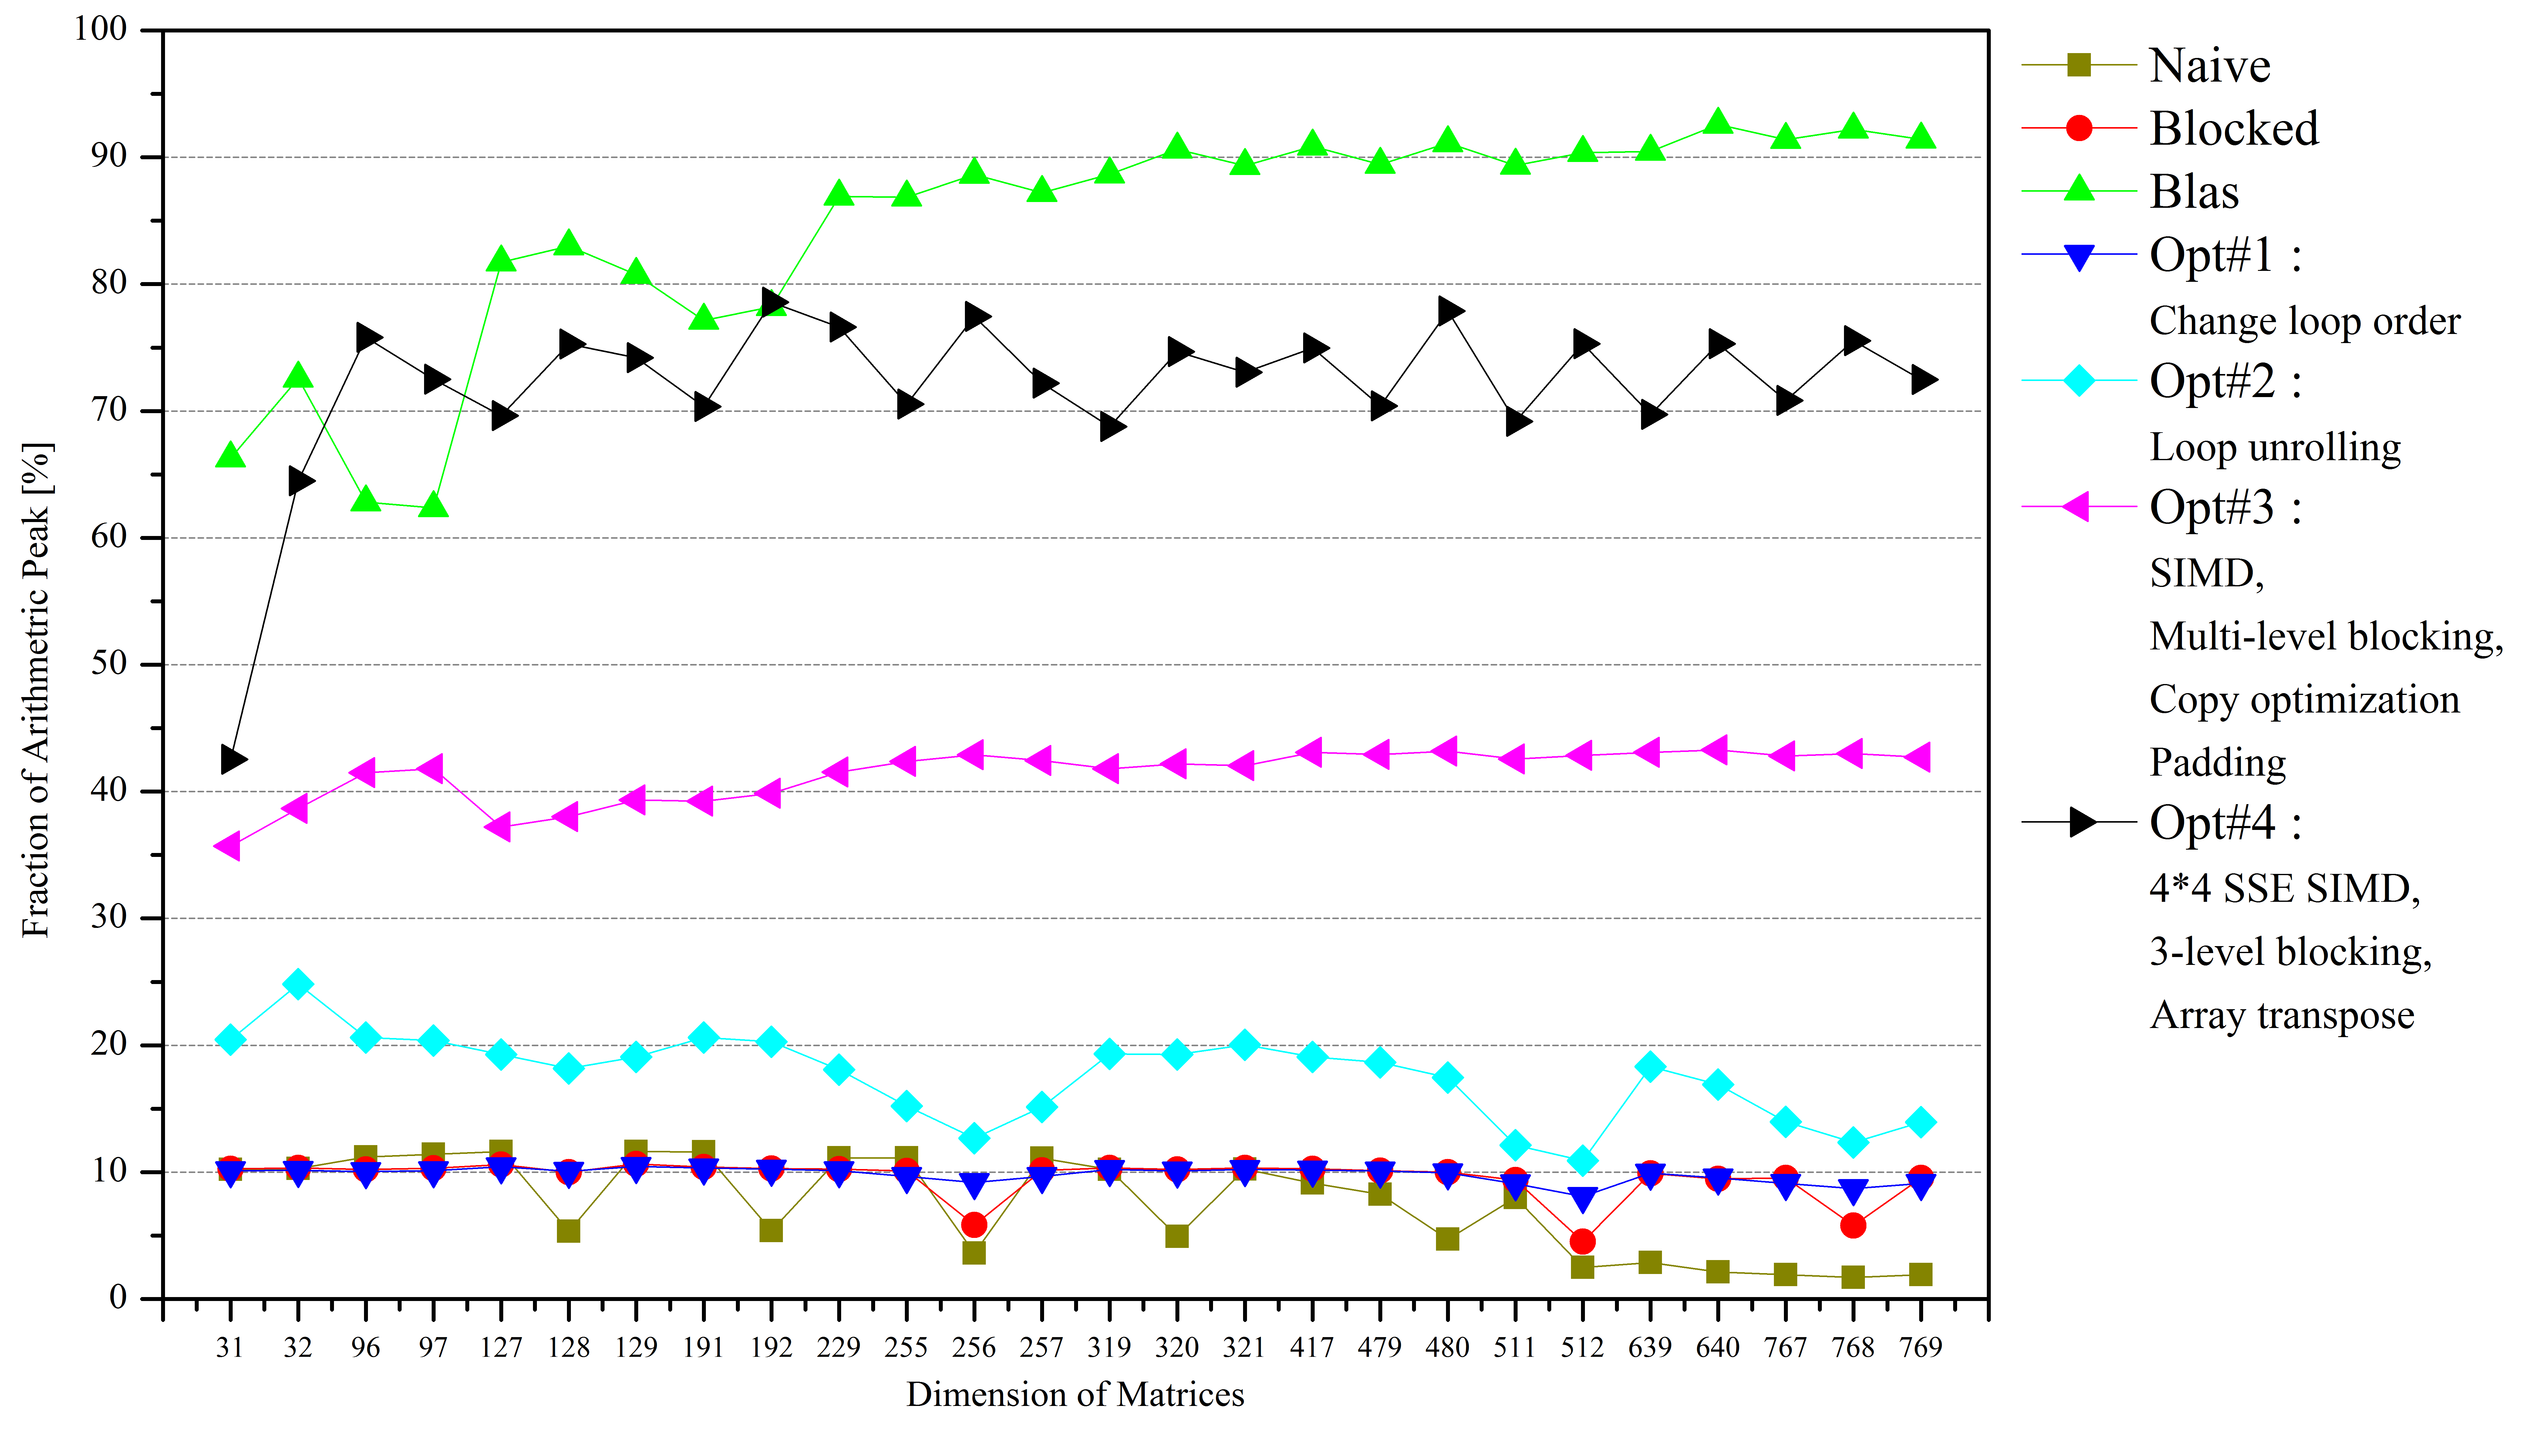
\includegraphics[width=1\columnwidth]{p1}
\caption{Matrix multiplication running results on Hopper from both references and different iterations of the optimized code, Team 11}
\label{p1}
\end{figure}
\end{homeworkSection}
%----------------------------------------------------------------------------------------
\begin{homeworkSection}{Exploration on compiler flags}
We tried different combination of compiler flags. In the end, besides -Ofast flags, we added:
\medskip
\\
\texttt{-funroll-loops}
\medskip
\\
Unroll loops whose number of iterations can be determined at compile time or upon entry to the loop. \texttt{-funroll-loops} implies \texttt{-frerun-cse-after-loop}, \texttt{-fweb} and \texttt{-frename-registers}. It also turns on complete loop peeling (i.e. complete removal of loops with a small constant number of iterations). This option makes code larger, and may or may not make it run faster.
\medskip
\\
\texttt{-ffast-math}
\\
Sets the options \texttt{-fno-math-errno}, \texttt{-funsafe-math-optimizations}, \texttt{-ffinite-math-only}, 
\\ \texttt{-fno-rounding-math}, \texttt{-fno-signaling-nans} and \texttt{-fcx-limited-range}. 
\\
This option causes the preprocessor macro \texttt{ \_\_FAST\_MATH\_\_} to be defined. 
\end{homeworkSection}
\end{section}
%------------------------------------------------------------------
\begin{section}{Running on a different machine}

The optimized code, at different iteration step is also run on a Macbook Pro laptop: Intel Core i7-3540M Processor (4M Cache, 3 GHz, turbo up to 3.70 GHz), 8GB DDR3 1333-MHz memory, Mac OS X 10.10.2 system. The result is shown in Figure \ref{p2}. The trend between iteration steps is the same as results from Hopper. For the most optimized code result, it is 80\% faster on this laptop than that on Hopper, mainly because the processor on the laptop has higher frequency and supports newer SSE instruction set. Note that the dips in performance are not exactly the same as Hooper's. The potential cause could be that the cache sizes on Core i7 and AMD Opteron.

\begin{figure}[!htb]
\centering
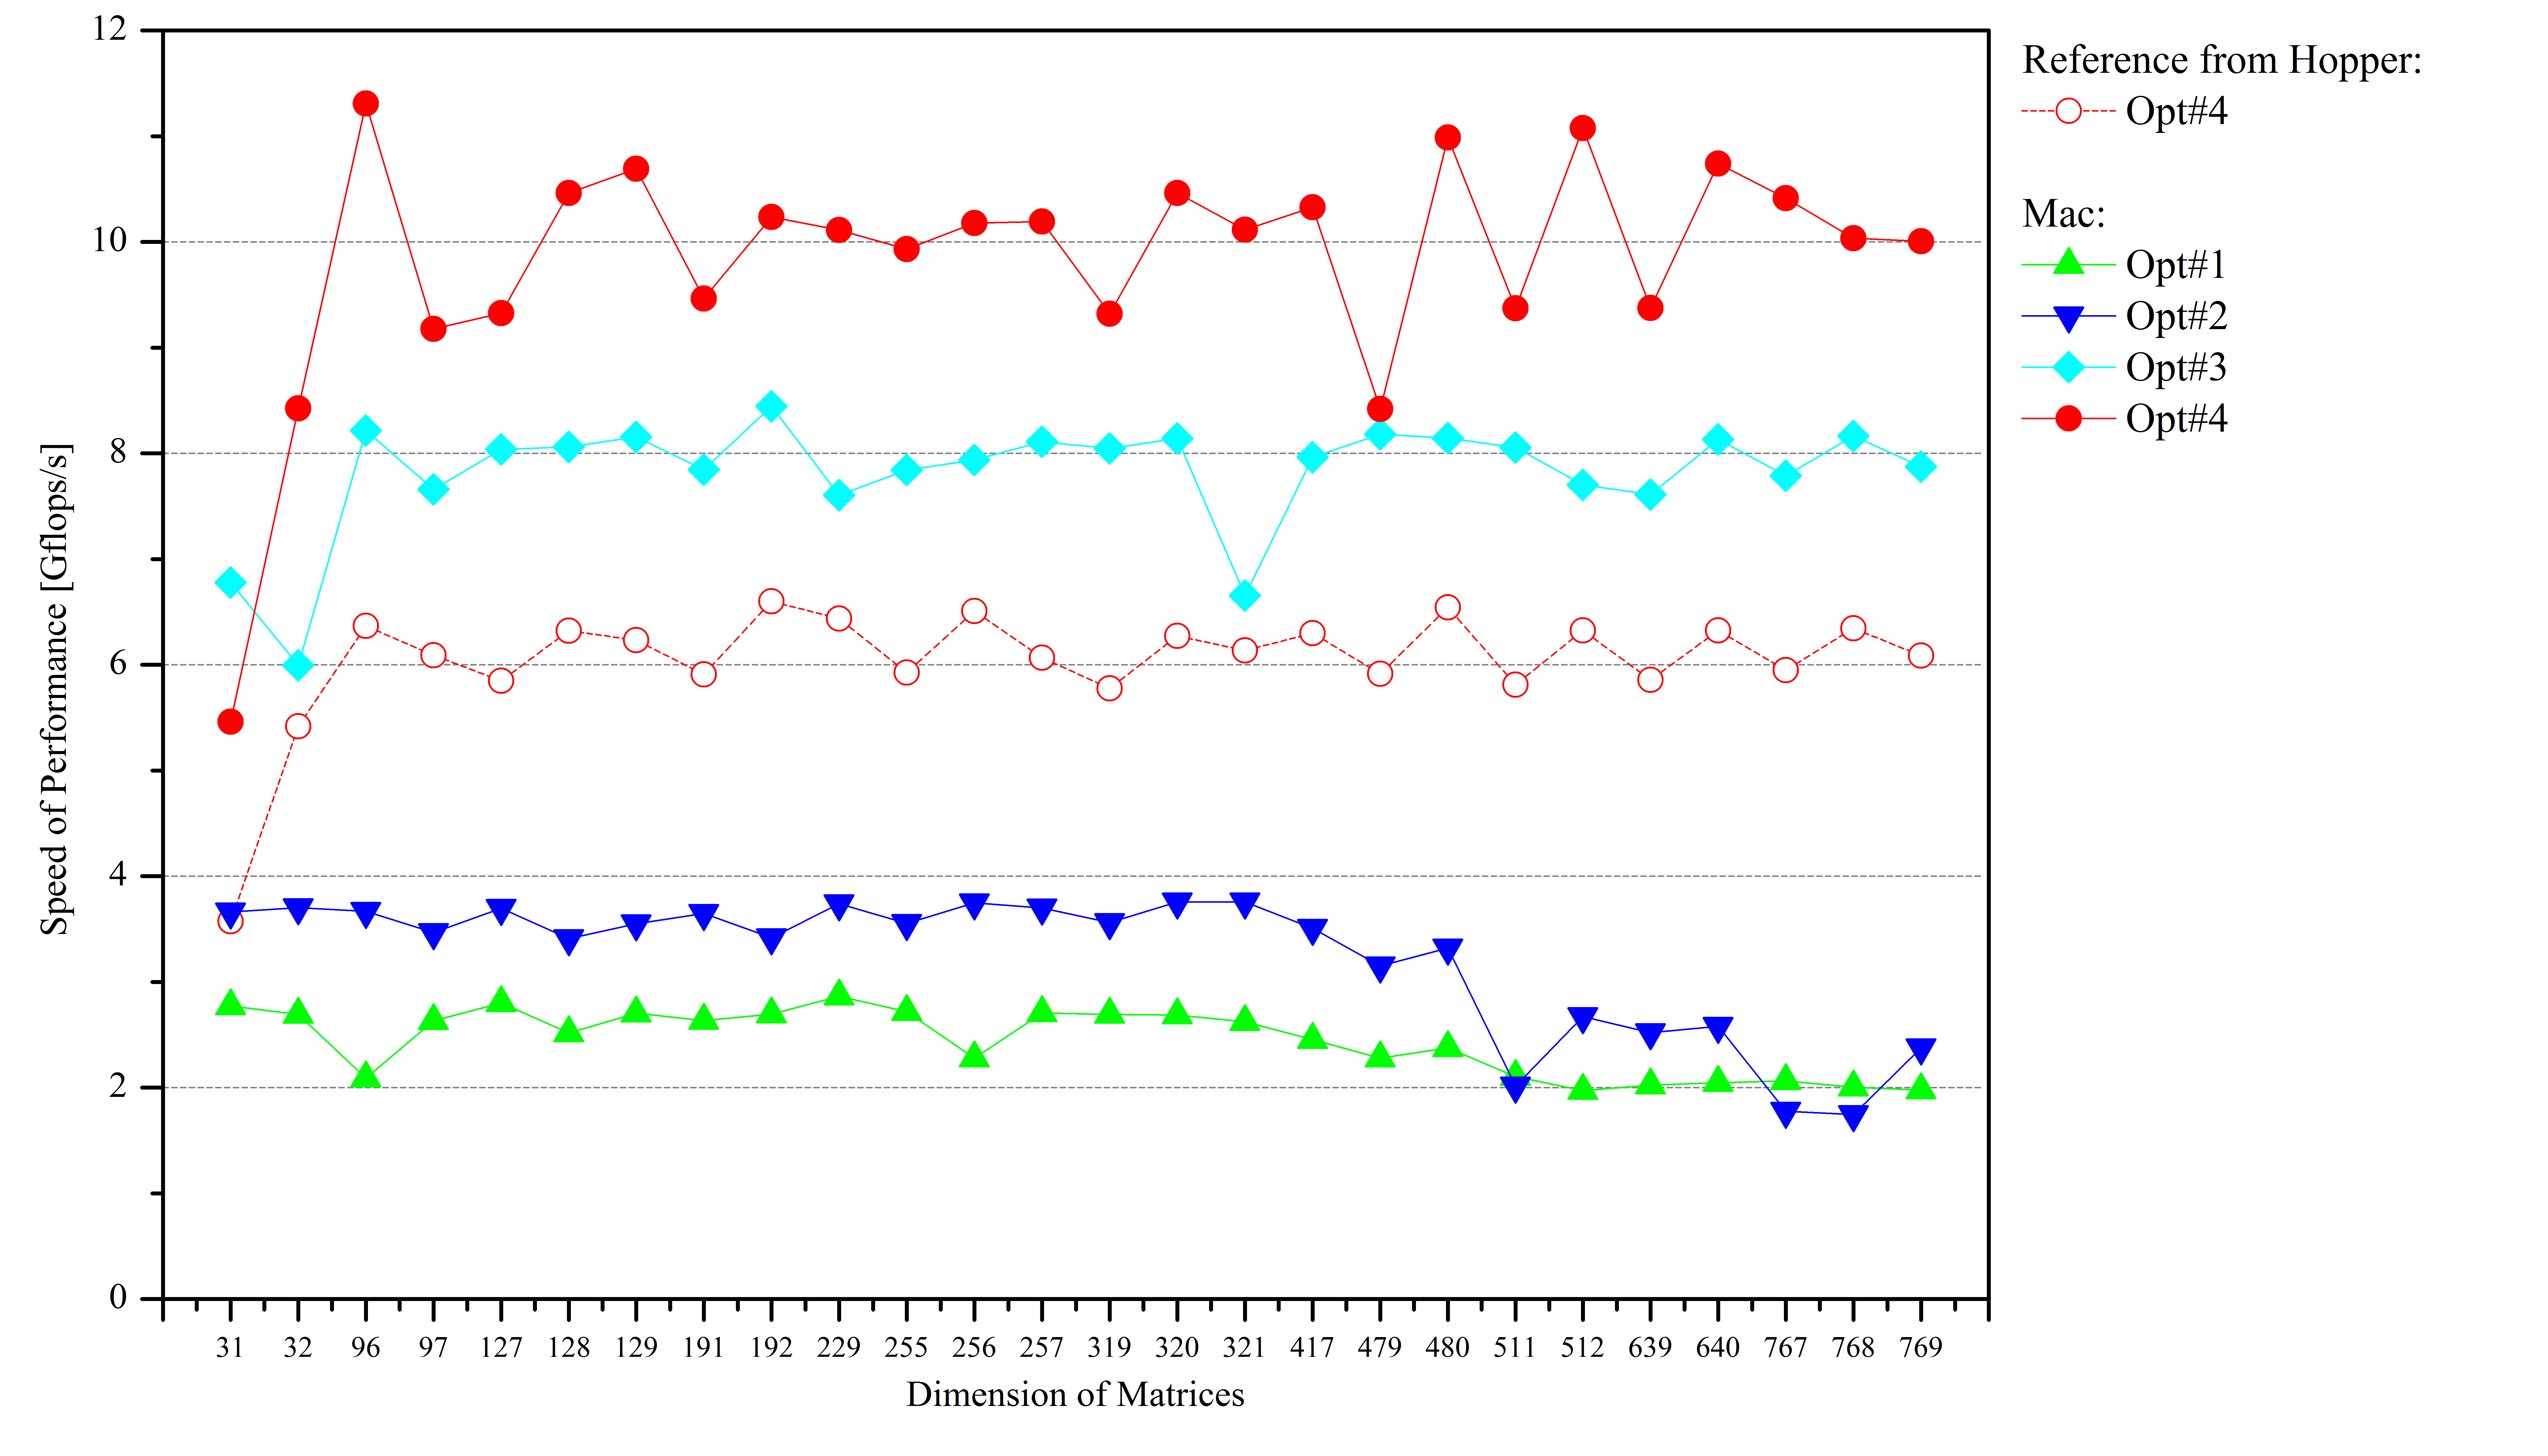
\includegraphics[width=1\columnwidth]{p2}
\caption{Matrix multiplication running results on Macbook, Team 11}
\label{p2}
\end{figure}
\end{section}
%------------------------------------------------------------------
\newpage
\begin{thebibliography}{9}
\bibitem{goto2008}
Goto, Kazushige, and Robert A. Geijn. Anatomy of high-performance matrix multiplication. \textit{ACM Transactions on Mathematical Software (TOMS)} 34.3 (2008): 12.
\bibitem{Abrash1997}
Abrash, Michael. \textit{Michael Abrash's Graphics Programming Black Book, with CD: The Complete Works of Graphics Master, Michael Abrash.} Coriolis group books, 1997.
\end{thebibliography}

\end{document}